\section{Rekursive Eigenschaft der Kugelvolumen\label{gamma:section:spheres}}
\kopfrechts{Kugelvolumen}

$\pi$ ist definiert als die Konstante, welche 
\eqref{gamma-eq:circumference} erfüllt.

\begin{equation}
\label{gamma-eq:circumference}
    2 \pi r = \text{Umfang eines Kreises mit dem Radius $r$}
\end{equation}

\noindent
Eine Kreisscheibe ist die von einem Kreisrand begrenzte, vollständig ausgefüllte Fläche eines Kreises.
Mit Hilfe von \eqref{gamma-eq:circumference} lässt sich die Fläche einer Kreisscheibe herleiten. 
Geht die Breite eines Rings gegen 0, verhält sich das 
Wachtstum des Flächeninhalts gleich wie das des Umfangs des Rings.
Das macht eine Herleitung der Kreisscheibenfläche per Integral, gezeigt in \eqref{gamma-eq:area}, möglich.
Für eine grafische Darstellung dieser 
Intuition siehe Abb. \ref{gamma-fig:ring-integration}.

\begin{equation}
\label{gamma-eq:area}
    A(r) = \int_{0}^{r} 2 \pi r \,dr = \pi r^2
\end{equation}

\noindent
Der Satz des Pythagoras gibt uns eine einfache Beschreibung aller 
Punkte, die Teil des Kreises sind \eqref{gamma-eq:pythagoras}.

\begin{equation}
\label{gamma-eq:pythagoras}
    x^2 + y^2 \leq r^2
\end{equation}

\noindent
Aufgrund der Ungleichung \eqref{gamma-eq:pythagoras} 
lässt sich eine weitere Definition der Kreisfläche herleiten, 
wenn wir sie nach $y$ auflösen \eqref{gamma-eq:pythagoras-y}
und für jedes $x$ den jeweils höchsten $y$-Wert integrieren
\eqref{gamma-eq:area-pythagoras}. Die Intuition dahinter wird
in Abb. \ref{gamma-fig:rect-integration} dargestellt.

\begin{gather}
\label{gamma-eq:pythagoras-y}
    y \leq \sqrt{r^2 - x^2} \\
\label{gamma-eq:area-pythagoras}
    A(r) = 2 \int_{-r}^{r} \sqrt{r^2-x^2} \,dx
\end{gather} 

\noindent
Das Integral aus \eqref{gamma-eq:area-pythagoras} ist nicht trivial 
zu lösen und wird nicht weiter verfolgt. Ein Vorteil ist, 
dass sich die durch den Satz des Pythagoras definierte Metrik 
einfach auf weitere Dimensionen erweitern lässt. 
\eqref{gamma-eq:pythagoras-3d} zeigt die Eweiterung in drei Dimensionen.

\begin{equation}
\label{gamma-eq:pythagoras-3d}
    \begin{split}
    x^2 + y^2 + z^2 \leq r^2 \\
    z \leq \sqrt{r^2 - x^2 - y^2}
    \end{split}
\end{equation}

\noindent
Nun können wir das Volumen einer Kugel herleiten, indem wir Halbkreise entsprechender
Grösse entlang $x$ integrieren (siehe Abb. \ref{gamma-fig:semicircle-integration}), während iterativ
in jedem Halbkreis entlang der $y$-Achse integriert wird.
Eine formelle Begründung für diese iterative angehensweise ist der Satz von Fubini.

\begin{figure}[h]
\centering
\subfigure[Integration unendlich dünner Ringe zur Berechnung der Fläche.\label{gamma-fig:ring-integration}]{%
    \begin{minipage}[c][4cm][c]{0.3\textwidth}
        \centering
        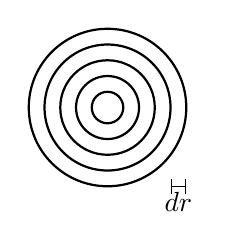
\begin{tikzpicture}
            \foreach \r in {0.2, 0.4, 0.6, 0.8, 1.0} {
                \draw[thick] (0,0) circle (\r cm);
            }
            \draw[{|}-{|}] (0.8,-1) -- (1.0, -1)
                node[midway, yshift=-.2cm] {$dr$};
        \end{tikzpicture}
    \end{minipage}%
}\hfill
\subfigure[Integration unendlich dünner Rechtecke zur Berechnung der Fläche.\label{gamma-fig:rect-integration}]{%
    \begin{minipage}[c][4cm][c]{0.3\textwidth}
        \centering
        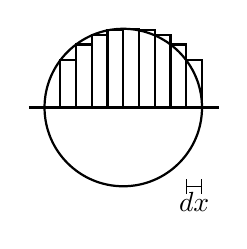
\begin{tikzpicture}
            \def\r{1}
            \draw[{|}-{|}] (0.8,-1) -- (1.0, -1)
                node[midway, yshift=-.2cm] {$dx$};

            \draw[thick] (0,0) circle (\r);
            \draw[thick] (-1.2,0) -- (1.2,0);
            \def\numrect{10}
            \pgfmathsetmacro\dx{2*\r/\numrect}
            \foreach \i in {0,1,...,\numrect} {
                \pgfmathsetmacro\x{-\r + \i*\dx}
                \pgfmathsetmacro\h{sqrt(max(0, \r*\r - \x*\x))}
                \draw[thick] (\x, 0) rectangle ++(\dx, \h);
            }
        \end{tikzpicture}
    \end{minipage}%
}\hfill
\subfigure[Integration von Halbkreisen zur Berechnung des Volumens.\label{gamma-fig:semicircle-integration}]{%
    \begin{minipage}[c][4cm][c]{0.3\textwidth}
        \centering
        \tdplotsetmaincoords{70}{25}
        \begin{tikzpicture}[tdplot_main_coords]
            \def\r{1}
            \def\numrect{8}
            \pgfmathsetmacro\dx{2*\r/\numrect}

            \draw[->] (-\r-0.5, 0, 0) -- (\r+0.5, 0, 0) node[anchor=north east] {$x$};
            \draw[->] (0, -\r-0.5, 0) -- (0, \r+0.5, 0) node[anchor=north west] {$y$};
            \draw[->] (0, 0, -\r-0.5) -- (0, 0, \r+0.5) node[anchor=south] {$z$};

            \foreach \i in {1,...,\numrect} {
                \pgfmathsetmacro\xc{-\r + \i*\dx - 0.5*\dx}
                \pgfmathsetmacro\sliceR{sqrt(max(0, \r*\r - \xc*\xc))}

                \pgfmathsetmacro\nextxc{-\r + (\i+1)*\dx - 0.5*\dx}

                \draw[black, thick, fill=black!10, fill opacity=0.4]
                    plot[domain=0:180, samples=40] ({\xc}, {\sliceR*cos(\x)}, {\sliceR*sin(\x)}) -- cycle;
                \draw[black, thick, fill=black!10, fill opacity=0.4]
                    plot[domain=0:180, samples=40] ({\nextxc}, {\sliceR*cos(\x)}, {\sliceR*sin(\x)}) -- cycle;
                \draw[black, thick] (\xc, \sliceR, 0) -- (\nextxc, \sliceR, 0);
                \draw[black, thick] (\xc, -\sliceR, 0) -- (\nextxc, -\sliceR, 0);
                \draw[black, thick] (\xc, 0.17*\sliceR, \sliceR) -- (\nextxc+0.05,  0.19*\sliceR, \sliceR);
            }

            % \draw[thick, gray] plot[domain=0:360, samples=60] ({\r*cos(\x)}, {\r*sin(\x)}, 0);
            % \draw[thick, gray] plot[domain=0:360, samples=60] ({\r*cos(\x)}, 0, {\r*sin(\x)});
            % \draw[thick, gray] plot[domain=0:360, samples=60] (0, {\r*cos(\x)}, {\r*sin(\x)});

            % dx measurement - aligned with the first slice
            \pgfmathsetmacro\firstX{-\r + 1*\dx - 0.5*\dx}
            \draw[|-|] (\firstX-\dx/2, 0, -\r-0.4) -- (\firstX+\dx/2, 0, -\r-0.4) node[midway, below] {$dx$};
        \end{tikzpicture}
    \end{minipage}%
}
\caption{Intuition hinter Integration über Raum}
\end{figure}


\noindent
Für ein bestimmtes $x$ sind die möglichen $y$-Werte gemäss Ungleichung 
\eqref{gamma-eq:pythagoras-y} eingeschränkt und für ein bestimmtes $x$ und $y$ wird dann
der maximale Wert für $z$ gemäss Ungleichung \eqref{gamma-eq:pythagoras-3d} genommen. 
Dies ist in \eqref{gamma-eq:sphere-volume} zu sehen.

\begin{equation}
\label{gamma-eq:sphere-volume}
    V(r) = 2 \int_{-r}^{r} \int_{-\sqrt{r^2-x^2}}^{\sqrt{r^2-x^2}} \sqrt{r^2-x^2-y^2} \,dy \,dx
\end{equation}

\noindent
Da wir aber bereits die Fläche eines Kreises berechnen können, können wir $A(r)$
zur Berechnung des Kugelvolumens anstatt der Pythagoras-Methode verwenden, wie in 
\eqref{gamma-eq:composed-sphere-volume}.

\begin{equation}
\label{gamma-eq:composed-sphere-volume}
    V(r) = 2 \int_{-r}^{r} A\left(\sqrt{r^2-x^2}\right) \,dx
\end{equation}

\noindent
Wir haben etwas interessantes getan, nämlich die Berechnung für zwei Dimensionen 
verwendet, um das Volumen in drei Dimensionen zu berechnen. 

Auf diese Weise lässt sich also das Volumen auf beliebige Dimensionen $> 2$ erweitern, und zwar 
mit \eqref{gamma-eq:n-sphere-volume-recursive}.

\begin{equation}
\label{gamma-eq:n-sphere-volume-recursive}
    V_{n+1}(r) = \int_{-r}^{r} V_n\left(\sqrt{r^2-x^2}\right) \,dx
\end{equation}

\noindent
Betrachtet man $A(r) = V_2(r) = 2 \pi r$, so scheint es intuitiv, dass $V_n$ jeweils mit $C_n r^n$
dargestellt werden kann, wobei $C_n$ eine der Dimension zugehörige Konstante ist.

Wir können induktiv beweisen, dass $V_{n+1}$ dieser Form entspricht, sofern
$V_n$ dieser Form entspricht, siehe~\eqref{gamma-eq:const-structure-induction}.

\begin{gather}
\label{gamma-eq:const-structure-induction}
    \text{Nehme an, dass } V_n(r) = C_n r^n \text{. Dann gilt:} \nonumber \\
    \begin{split}
         V_{n+1}(r) &= \int_{-r}^{r} C_n \left(\sqrt{r^2-x^2}\right)^n \,dx  \\ 
        &= \int_{-r}^{r} C_n \left(r^2-x^2\right)^{n/2} \,dx \\
        &= \int_{-1}^{1} C_n \left(r^2 - (ru)^2\right)^{n/2} r \,du \\
        &= \int_{-1}^{1} C_n \left(r^2 (1 - u^2)\right)^{n/2} r \,du \\
        &= \int_{-1}^{1} C_n r^{n+1} (1- u^2)^{n/2} \,du \\
        &= r^{n+1} \underbrace{C_n \int_{-1}^{1} (1- u^2)^{n/2} \,du}_{C_{n+1}} \\
    \end{split}
\end{gather}

\noindent
Wir sehen, dass $C_n$ ein Faktor von $C_{n+1}$ ist. Die mit dem Volumen assoziierte Konstante 
scheint also eine rekursive Struktur ähnlich der einer Fakultät aufzuweisen. Eine Untersuchung des Terms $I_n = \int_{-1}^1 (1- u^2)^{n/2} \,du$ in \eqref{gamma-eq:n-sphere-constant} ergibt eine weitere rekursive Struktur: $I_n = \frac{n}{n+1} I_{n-2}$.

\begin{equation}
\label{gamma-eq:n-sphere-constant}
    \begin{split}
        I_n &= \int_{-1}^1 (1- u^2)^{n/2} \,du \\
        &= \left[ u (1-u^2)^{n/2} \right]_{-1}^{1} - \int_{-1}^1 u \cdot (-nu(1-u^2)^{n/2 - 1}) \,du \\
        &= (0 - 0) - \int_{-1}^1 -nu^2(1-u^2)^{n/2 - 1} \,du \\
        &= n \int_{-1}^1 u^2 (1 - u^2)^{n/2 - 1} \,du \\
        &= n \int_{-1}^1 (1 - (1 - u^2)) (1-u^2)^{n/2 - 1} \,du \\
        &= n \int_{-1}^1 (1 - u^2)^{n/2 - 1} \,du - n \int_{-1}^1 (1-u^2)^{n/2} \,du \\
        &= n I_{n-2} - n I_n \\
        (n+1) I_n &= n I_{n-2} \\
        I_n &= \frac{n}{n+1} I_{n-2} \\
    \end{split}
\end{equation}

\noindent
Mit diesem Wissen lässt sich der konstante Faktor des Volumens einer
$n$-Dimensionalen Kugel herleiten als $C_n = C_{n-1} I_{n-1} = C_{n-2} I_{n-1}
I_{n-2} = C_{n-2} \frac{2}{n} I_1 I_0$. Der letzte Schritt ist
durch~\eqref{gamma-eq:n-sphere-constant-2} begründet, funktioniert aber nur mit
geraden $n$.

\begin{equation}
\label{gamma-eq:n-sphere-constant-2}
    \begin{split}
    I_{n-1} I_{n-2} &= (\frac{n-1}{n} \cdot \frac{n-3}{n-2} \cdot \ldots \cdot \frac{3}{4} \cdot I_1) \cdot (\frac{n-2}{n-1} \cdot \frac{n-4}{n-2} \cdot \ldots \cdot \frac{2}{3} \cdot I_0) \\
    &= \frac{n-1}{n} \cdot \frac{n}{n-1} \cdot \ldots \cdot \frac{3}{4} \cdot  \frac{2}{3} \cdot I_1 I_0 \\
    &= \frac{2}{n} \cdot I_1 I_0
    \end{split}
\end{equation}

\noindent
Von~\eqref{gamma-eq:area} wissen wir, dass $C_2 = \pi$. Eine einfache Rechnung
ergibt, dass $I_0 = 2$ und $I_1 = \frac{\pi}{2}$, d.h. $C_n = C_{n-2} \frac{2 \pi}{n}$. Jetzt können wir für gerade Dimensionen
die rekursive Definition `abrollen' in einen einzigen
Term:~\eqref{gamma-eq:nonrecursive-constant}.

\begin{equation}
\label{gamma-eq:nonrecursive-constant}
    \begin{split}
        C_n &= \pi \cdot \frac{2 \pi}{4} \cdot \frac{2 \pi}{6} \cdot \ldots \cdot \frac{2 \pi}{n} \\
            &= \frac{2 \pi}{2} \cdot \frac{2 \pi}{4} \cdot \frac{2 \pi}{6} \cdot \ldots \cdot \frac{2 \pi}{n} \\
            &= \frac{(2 \pi)^{n/2}}{2^{n/2}} \frac{1}{\left(\frac{n}{2}\right)!} \\
            &= \frac{\pi^{n/2}}{\left(\frac{n}{2}\right)!}
    \end{split}
\end{equation}

\noindent
Wir können jetzt also wie in \eqref{gamma-eq:n-sphere-volume-even} ein Kugelvolumen bei geraden Dimensionen einfach berechnen.

\begin{equation}
\label{gamma-eq:n-sphere-volume-even}
    V_n(r) = \frac{\pi^{n/2}}{(\frac{n}{2})!}  r^n
\end{equation}

\noindent
Schön wäre es, das Volumen nicht nur für gerade-Dimensionale Kugeln berechnen können. 
Dazu müssten wir allerdings die Fakultät auf halbe Zahlen anwenden können, was einer der Gründe ist die Fakultät zu erweitern.
